\documentclass[11pt]{article}

\usepackage[a4paper,margin=26mm]{geometry}
\usepackage[T1]{fontenc}
\usepackage[utf8]{inputenc}
\usepackage{lmodern}
\usepackage{microtype}
\usepackage{amsmath,amssymb,amsthm,mathtools,bm}
\usepackage{enumitem}
\usepackage{xcolor}
\usepackage{tikz}
\usetikzlibrary{positioning,arrows.meta,calc,decorations.pathreplacing}
\usepackage{hyperref}
\usepackage[nameinlink,noabbrev]{cleveref}

\hypersetup{
  colorlinks=true,
  linkcolor=blue!55!black,
  citecolor=blue!55!black,
  urlcolor=blue!55!black,
  pdftitle={Optimal Unambiguous Dual-Rail Bell-State Measurement with Linear Optics and Two Ancillary Photons},
  pdfauthor={Mansehej Singh}
}

\newtheorem{theorem}{Theorem}
\newtheorem{lemma}[theorem]{Lemma}
\newtheorem{proposition}[theorem]{Proposition}
\newtheorem{corollary}[theorem]{Corollary}
\theoremstyle{remark}
\newtheorem{remark}[theorem]{Remark}
\newtheorem{definition}[theorem]{Definition}

\newcommand{\ket}[1]{\lvert #1\rangle}
\newcommand{\bra}[1]{\langle #1\rvert}
\newcommand{\braket}[2]{\langle #1\mid #2\rangle}
\newcommand{\abs}[1]{\lvert #1\rvert}
\newcommand{\norm}[1]{\lVert #1\rVert}
\newcommand{\Id}{\mathbb{I}}
\newcommand{\diag}{\operatorname{diag}}
\newcommand{\Tr}{\operatorname{Tr}}
\newcommand{\psucc}{P_{\mathrm{succ}}}
\newcommand{\Pstar}{P_2^\star}

\title{\textbf{Optimal Unambiguous Dual-Rail Bell-State Measurement with Linear Optics and Two Ancillary Photons}}
\author{Mansehej Singh\\[2pt]
  \normalsize Independent Researcher\\[1pt]
  \normalsize\texttt{mansehej@gmail.com}}
\date{19 August 2026}

\begin{document}
\maketitle

\begin{abstract}
We determine the exact optimum for unambiguous discrimination of the four
dual-rail photonic Bell states using a single static passive interferometer,
ideal photon-number-resolving detection, arbitrary vacuum extensions, and an
arbitrary normalized pure ancillary state containing exactly two photons. No
polarization-preserving restriction, product-state assumption, fixed mode
count, or canonical interferometer ansatz is imposed. For each output mode we
remove one detected photon and form a conditional Gram matrix. Exact
unambiguous outcomes identify exclusive Fock components; deleting these
components leaves a positive-semidefinite residual Gram matrix. A product state
can always be chosen in the kernel of the pulled-back signal annihilator, and
its squared overlaps with the Bell basis are at most one half. These facts give
a per-mode success budget which, after summing over output modes and using
photon-number conservation, yields
\(P_{\mathrm{succ}}\le 3/4\). The two-photon construction of Grice attains
the bound, so \(P_2^\star=3/4\). More generally, the same argument gives the
fixed-\(k\)-photon upper bound
\(P_{\mathrm{succ}}\le (k+1)/(k+2)\). Combined with the recursive
constructions of Grice, this determines the exact optimum
\(P_k^\star=1-2^{-N}\) for every ancillary photon number \(k=2^N-2\).
\end{abstract}

\section{Introduction}

Bell-state measurements are central to quantum teleportation, entanglement
swapping, photonic fusion gates, and optical quantum
repeaters~\cite{Bartolucci2023}. Their static linear-optical implementation
is limited because passive mode transformations cannot create a direct
photon--photon interaction. Perfect discrimination of the four dual-rail
Bell states is impossible with linear
optics~\cite{Vaidman1999,Lutkenhaus1999}, and with only vacuum auxiliary
modes, unambiguous discrimination of equiprobable dual-rail Bell states cannot
exceed one half~\cite{Calsamiglia2001}. Populated ancillary states change the
problem: Grice exhibited an entangled two-photon ancilla reaching
\(3/4\)~\cite{Grice2011}, while Ewert and van Loock reached \(3/4\) using four
externally unentangled ancillary photons and obtained \(5/8\) in the relevant
two-extra-photon truncation~\cite{Ewert2014}. Both regimes have been probed
experimentally: a boosted Bell-state measurement with two unentangled
ancillary photons reached \(57.9\%\)~\cite{Bayerbach2023}, and one with an
ancillary Bell pair reached \(69.3\%\)~\cite{Hauser2024}. Active resources
change the problem again---already single-mode squeezing beats one half with
no ancillary photon at all~\cite{Zaidi2013}---but lie outside the static
passive model considered here.

The unresolved point is the resource-complete upper bound. For
interferometers that preserve polarization, Olivo and Grosshans proved the
upper bound \((k+1)/(k+2)\) for even ancillary photon number \(k\)---the same
value established here---and their numerical searches over unrestricted
networks plateaued at \(3/4\) for a two-photon ancilla; for optimality beyond
the polarization-preserving class they reported ``evidences (but no
proofs)''~\cite{Olivo2018}. A recent review likewise records the analytical
bound only in its polarization-preserving form~\cite{Bianchi2025}. Work on
auxiliary degrees of freedom carried by the same two photons addresses a
different, ancilla-photon-free resource model~\cite{Laha2026}.

This paper closes the exactly-two-ancillary-photon problem without restricting
the number of ancillary or vacuum modes and without restricting the passive
unitary; in particular, no polarization-preserving structure is assumed. The proof is dimension independent and depends only on (i) exact
unambiguity, (ii) fixed photon number, (iii) the maximally mixed one-particle
reduced density matrix of every Bell input, and (iv) the product geometry of the
dual-rail signal subspace.


\section{Resource model}
\label{sec:model}

The four signal modes contain one of the equiprobable Bell states
\begin{align}
\ket{\Phi^\pm}
  &=\frac{a_1^\dagger a_3^\dagger\pm a_2^\dagger a_4^\dagger}{\sqrt2}\ket0,
  \\
\ket{\Psi^\pm}
  &=\frac{a_1^\dagger a_4^\dagger\pm a_2^\dagger a_3^\dagger}{\sqrt2}\ket0.
\end{align}
We write these in the fixed order
\[
\ket{B_1}=\ket{\Phi^+},\quad
\ket{B_2}=\ket{\Phi^-},\quad
\ket{B_3}=\ket{\Psi^+},\quad
\ket{B_4}=\ket{\Psi^-}.
\]

Let the ancillary input be an arbitrary normalized pure state of exactly two
photons in \(r\) additional modes,
\begin{equation}
  \ket\chi_A=\sum_{\nu:\,|\nu|=2}\chi_\nu\ket\nu,
  \qquad \sum_{\nu}\abs{\chi_\nu}^2=1,
\end{equation}
where repeated occupation of a mode is allowed. Let \(v\) further modes enter
in vacuum. Thus the total number of modes is \(m=4+r+v\), with no a priori
upper bound except finiteness.

A passive interferometer \(U\in U(m)\) acts once on all modes. It is followed
by ideal photon-number-resolving (PNR) detection in every output mode. There is
no feed-forward, squeezing, nonlinearity, intermediate destructive
measurement, auxiliary degree of freedom, or additional populated photon.

For label \(j\), define the output state
\begin{equation}
  \ket{\Omega_j}
   =\mathcal U\bigl(\ket{B_j}_S\ket\chi_A\ket0_V\bigr),
  \qquad
  A_j(n)=\braket{n}{\Omega_j},
\end{equation}
where every occupation \(n=(n_1,\ldots,n_m)\) in the support satisfies
\(\sum_\ell n_\ell=4\).

A set \(S_j\) of occupations is a valid successful set for label \(j\) if
\begin{equation}
  n\in S_j,\ k\ne j \quad\Longrightarrow\quad A_k(n)=0.
  \label{eq:unambiguous}
\end{equation}
Successful sets may omit otherwise exclusive outcomes, but they may not overlap.
The conditional and average success probabilities are
\begin{equation}
  p_j=\sum_{n\in S_j}\abs{A_j(n)}^2,
  \qquad
  \psucc=\frac14\sum_{j=1}^4p_j.
\end{equation}
The optimization supremum over all allowed finite \(r,v,U,\chi\), and
assignments is denoted \(\Pstar\).

\begin{remark}[Generality of the model]
\label{rem:generality}
Three standard extensions are implicit. First, ideal PNR detection of every
output mode is the finest measurement available after a static passive
unitary; a protocol that discards modes, bins outcomes, or uses threshold
detectors observes a coarse-graining of the PNR statistics, and each of its
unambiguous outcomes lifts to a valid successful set of PNR patterns with
the same success probability. Second, a mixed two-photon ancilla cannot
help: exact unambiguity must hold separately for every pure state in the
support of the mixture, so the success probability is a convex average of
pure-ancilla success probabilities, each bounded by \cref{thm:main}. Third,
ancillary states without a definite photon number, such as coherent or
squeezed states, lie outside the model; the proof uses photon-number
conservation, and the corresponding optimum remains open.
\end{remark}



\section{Conditional Gram matrices}
\label{sec:gram}

Fix an output mode \(\ell\), with annihilation operator \(b_\ell\). Pull it
through the passive interferometer,
\begin{equation}
  c_\ell=\mathcal U^\dagger b_\ell\mathcal U.
\end{equation}
Because \(\mathcal U\) is passive, \(c_\ell\) is a linear combination of input
annihilation operators. Decompose its one-particle vector according to the
orthogonal input-mode sectors,
\begin{equation}
  c_\ell=s_\ell+r_\ell+v_\ell,
\end{equation}
where \(s_\ell\) acts on the four signal modes, \(r_\ell\) on the ancillary
modes, and \(v_\ell\) on the vacuum modes. The vacuum component annihilates the
input. Define the conditional three-photon states
\begin{equation}
  \ket{\phi_{j\ell}}
   =c_\ell\ket{B_j}_S\ket\chi_A\ket0_V.
\end{equation}
Their Gram matrix is \(G^{(\ell)}_{jk}=\braket{\phi_{j\ell}}{\phi_{k\ell}}\).

\begin{lemma}[Conditional Gram decomposition]
\label{lem:gram}
For every output mode \(\ell\),
\begin{equation}
  G^{(\ell)}_{jk}
   =\bra{B_j}s_\ell^\dagger s_\ell\ket{B_k}
     +q_\ell\delta_{jk},
  \qquad
  q_\ell:=\bra\chi r_\ell^\dagger r_\ell\ket\chi\ge0.
  \label{eq:gramdecomp}
\end{equation}
If \(t_\ell:=\norm{s_\ell}^2\) is the squared norm of the signal coefficient
vector, then
\begin{equation}
  G^{(\ell)}_{jj}=q_\ell+\frac{t_\ell}{2}
  \qquad (j=1,\ldots,4).
  \label{eq:gramdiag}
\end{equation}
\end{lemma}

\begin{proof}
The state obtained by applying \(s_\ell\) has signal/ancilla photon numbers
\((1,2)\), whereas the state obtained by applying \(r_\ell\) has photon numbers
\((2,1)\). These sectors are orthogonal, so the cross terms vanish. The
ancillary-annihilation term factors as
\(\braket{B_j}{B_k}\bra\chi r_\ell^\dagger r_\ell\ket\chi\), giving
\cref{eq:gramdecomp}. Every Bell state above has signal one-particle reduced
density matrix \(\Id_4/2\), hence
\(\bra{B_j}s_\ell^\dagger s_\ell\ket{B_j}=\norm{s_\ell}^2/2\), proving
\cref{eq:gramdiag}.
\end{proof}

\section{Exclusive outcomes and the residual Gram matrix}
\label{sec:deletion}

Define the successful photon weight in mode \(\ell\) by
\begin{equation}
  d_{j\ell}:=\sum_{n\in S_j}n_\ell\abs{A_j(n)}^2.
  \label{eq:ddef}
\end{equation}
On the output side,
\begin{equation}
  b_\ell\ket{\Omega_j}
   =\sum_{n:\,n_\ell>0}\sqrt{n_\ell}\,A_j(n)\ket{n-e_\ell}.
  \label{eq:annihilated-output}
\end{equation}

\begin{lemma}[Exclusive-component deletion]
\label{lem:delete}
For every \(\ell\),
\begin{equation}
  F_\ell:=G^{(\ell)}-D_\ell\succeq0,
  \qquad
  D_\ell:=\diag(d_{1\ell},d_{2\ell},d_{3\ell},d_{4\ell}).
  \label{eq:Fpsd}
\end{equation}
Consequently, with
\begin{equation}
  f_{j\ell}:=(F_\ell)_{jj}
    =q_\ell+\frac{t_\ell}{2}-d_{j\ell},
  \label{eq:fdef}
\end{equation}
we have \(f_{j\ell}\ge0\).
\end{lemma}

\begin{proof}
For fixed \(\ell\), the map \(n\mapsto n-e_\ell\) is injective on occupations
with \(n_\ell>0\): adding \(e_\ell\) recovers \(n\). If \(n\in S_j\), exact
unambiguity~\cref{eq:unambiguous} says that the coefficient of the same full
occupation \(n\) is zero for every \(k\ne j\). Hence the residual Fock basis
vector \(\ket{n-e_\ell}\) in \cref{eq:annihilated-output} is an exclusive
component of conditional vector \(j\).

Project all four conditional vectors orthogonally away from the span of every
such exclusive residual basis vector. The remaining vectors have a genuine
Gram matrix and therefore a positive-semidefinite one. Injectivity prevents
cross-counting, while exclusivity means that deleting these coordinates changes
only diagonal entry \(j\) by
\(\sum_{n\in S_j}n_\ell\abs{A_j(n)}^2=d_{j\ell}\). The residual Gram matrix is
therefore exactly \(F_\ell\), proving \cref{eq:Fpsd}. Nonnegativity of its
diagonal gives \(f_{j\ell}\ge0\).
\end{proof}

\section{A product-kernel vector and the per-mode budget}
\label{sec:permode}

Write the signal annihilator according to the two dual rails,
\begin{equation}
  s_\ell
  =\alpha_1a_1+\alpha_2a_2+\beta_1a_3+\beta_2a_4.
\end{equation}
Choose a normalized qubit vector \(\ket x_A\) in the kernel of the linear
functional \((\alpha_1,\alpha_2)\), and independently choose normalized
\(\ket y_B\) in the kernel of \((\beta_1,\beta_2)\). If either coefficient
pair vanishes, choose the corresponding qubit vector arbitrarily. The two
terms produced by annihilating a photon from the two rails lie in orthogonal
one-photon sectors, and each coefficient is zero by construction. Therefore
\begin{equation}
  s_\ell\ket x_A\ket y_B=0.
  \label{eq:productkernel}
\end{equation}
Expand this normalized product state in the Bell basis,
\begin{equation}
  \ket x_A\ket y_B=\sum_{j=1}^4 z_j\ket{B_j},
  \qquad
  w_j:=\abs{z_j}^2.
  \label{eq:bellweights}
\end{equation}
Because the Bell basis is orthonormal, \(\sum_jw_j=1\). Each Bell state has
Schmidt coefficients \((1/\sqrt2,1/\sqrt2)\), so its squared overlap with a
normalized product state is at most \(1/2\):
\begin{equation}
  0\le w_j\le\frac12.
  \label{eq:weightcap}
\end{equation}
Let \(G^{S,(\ell)}\) denote the first term in \cref{eq:gramdecomp}.
\Cref{eq:productkernel} implies \(G^{S,(\ell)}z=0\).

\begin{proposition}[Per-output-mode success budget]
\label{prop:permode}
For every output mode \(\ell\),
\begin{equation}
  \boxed{\sum_{j=1}^4d_{j\ell}\le4q_\ell+t_\ell.}
  \label{eq:permode}
\end{equation}
\end{proposition}

\begin{proof}
Since \(F_\ell\succeq0\), \cref{eq:productkernel,eq:bellweights} give
\begin{equation}
  0\le z^\dagger F_\ell z
   =q_\ell-\sum_{j=1}^4d_{j\ell}w_j.
  \label{eq:psdquad}
\end{equation}
Using \cref{eq:fdef} and \(\sum_jw_j=1\), this is equivalent to
\begin{equation}
  \sum_{j=1}^4f_{j\ell}w_j\ge\frac{t_\ell}{2}.
  \label{eq:weightedlower}
\end{equation}
On the other hand, \(f_{j\ell}\ge0\) and \(w_j\le1/2\) imply
\begin{equation}
  \sum_{j=1}^4f_{j\ell}w_j
   \le\frac12\sum_{j=1}^4f_{j\ell}.
\end{equation}
Thus \(\sum_jf_{j\ell}\ge t_\ell\). Summing \cref{eq:fdef} over \(j\) now
gives
\begin{align}
  \sum_jd_{j\ell}
   &=4q_\ell+2t_\ell-\sum_jf_{j\ell}
    \le4q_\ell+t_\ell,
\end{align}
which is \cref{eq:permode}.
\end{proof}


\section{Global optimum}
\label{sec:global}

\begin{theorem}[Two ancillary photons]
\label{thm:main}
For every protocol in the resource model of \cref{sec:model},
\begin{equation}
  \psucc\le\frac34.
\end{equation}
The bound is attained by a finite static passive circuit, and therefore
\begin{equation}
  \boxed{\Pstar=\frac34.}
\end{equation}
\end{theorem}

\begin{proof}
First sum the left side of \cref{eq:permode} over all output modes. Every
successful occupation contains exactly four photons, so
\begin{align}
  \sum_{\ell=1}^m\sum_{j=1}^4d_{j\ell}
   &=\sum_{j=1}^4\sum_{n\in S_j}
     \left(\sum_{\ell=1}^mn_\ell\right)\abs{A_j(n)}^2 \\
   &=4\sum_{j=1}^4p_j.
  \label{eq:leftglobal}
\end{align}

The pulled-back output annihilators form an orthonormal one-particle basis.
The squared norms of their projections onto the four-dimensional signal
one-particle subspace therefore satisfy the Parseval identity
\begin{equation}
  \sum_{\ell=1}^mt_\ell=4.
  \label{eq:tsum}
\end{equation}
Likewise the ancillary projections resolve the ancillary number operator:
\begin{equation}
  \sum_{\ell=1}^mq_\ell
   =\bra\chi N_A\ket\chi=2.
  \label{eq:qsum}
\end{equation}
Summing \cref{eq:permode} and applying
\cref{eq:leftglobal,eq:tsum,eq:qsum} yields
\begin{equation}
  4\sum_{j=1}^4p_j\le4(2)+4=12.
\end{equation}
Hence \(\sum_jp_j\le3\), and with equal priors
\(\psucc=\frac14\sum_jp_j\le3/4\).

The exact Grice circuit in \cref{sec:grice} has average success \(3/4\), so the
upper bound is attained. Since a finite protocol attains it, the supremum is a
maximum.
\end{proof}

\begin{corollary}[Fixed ancillary photon number]
\label{cor:k}
For an arbitrary normalized pure ancilla containing exactly \(k\) photons,
with all other assumptions unchanged,
\begin{equation}
  \psucc\le\frac{k+1}{k+2}.
  \label{eq:kbound}
\end{equation}
\end{corollary}

\begin{proof}
The per-mode proof is unchanged. Now every output contains \(k+2\) photons,
\(\sum_\ell q_\ell=k\), and \(\sum_\ell t_\ell=4\). Therefore
\begin{equation}
  (k+2)\sum_jp_j\le4k+4=4(k+1).
\end{equation}
Dividing by \(4(k+2)\) gives \cref{eq:kbound}.
\end{proof}

\begin{corollary}[Optimality of the Grice hierarchy]
\label{cor:hierarchy}
For every integer \(N\ge1\), let \(P_k^\star\) denote the optimum of the
resource model of \cref{sec:model} with the two-photon ancilla replaced by an
arbitrary normalized pure ancilla of exactly \(k\) photons. Then, for
\(k=2^N-2\),
\begin{equation}
  P_k^\star=\frac{k+1}{k+2}=1-2^{-N}.
\end{equation}
\end{corollary}

\begin{proof}
The recursive construction of Grice uses a static passive interferometer,
ideal PNR detection, and a pure entangled ancilla of exactly \(2^N-2\)
photons, and attains average success \(1-2^{-N}\)~\cite{Grice2011}.
\Cref{cor:k} supplies the matching upper bound.
\end{proof}

\begin{remark}
At \(k=0\), \cref{eq:kbound} reproduces the vacuum-ancilla \(1/2\)
limit~\cite{Calsamiglia2001}; at \(k=2\), it is \cref{thm:main}. For odd
\(k\) the bound is unlikely to be tight: within polarization-preserving
networks the stronger bound \(P_{\mathrm{succ}}\le k/(k+1)\)
holds~\cite{Olivo2018}, and no construction exceeding \(k/(k+1)\) is known
at any odd \(k\).
\end{remark}

\section{Attainment by the Grice construction}
\label{sec:grice}

Use eight modes in the order
\begin{equation}
  (H_1,V_1,H_2,V_2,H_3,V_3,H_4,V_4),
\end{equation}
with the first four modes carrying the two input qubits and the last four the
ancilla. The normalized ancillary state is
\begin{equation}
  \ket{\chi_G}
   =\frac{a_5^\dagger a_7^\dagger+a_6^\dagger a_8^\dagger}{\sqrt2}\ket0.
  \label{eq:griceanc}
\end{equation}
On the four spatial paths, apply
\begin{equation}
  S=\frac12
  \begin{pmatrix}
  1&i&i&-1\\
  i&1&-1&i\\
  i&-1&1&i\\
  -1&i&i&1
  \end{pmatrix}
  \label{eq:S}
\end{equation}
identically to both rails. Equivalently, in path-major mode ordering,
\begin{equation}
  U_{(p,\rho),(q,\sigma)}=S_{pq}\delta_{\rho\sigma}.
\end{equation}
The matrix is exactly unitary. Moreover,
\begin{equation}
  S=B\otimes B,
  \qquad
  B=\frac1{\sqrt2}\begin{pmatrix}1&i\\ i&1\end{pmatrix},
  \label{eq:BS}
\end{equation}
so a passive decomposition uses two layers of balanced beam splitters. In the
full eight-mode ordering, the layers act on mode pairs
\begin{align}
  &(1,5),(2,6),(3,7),(4,8),\\
  &(1,3),(2,4),(5,7),(6,8).
\end{align}

\begin{figure}[t]
\centering
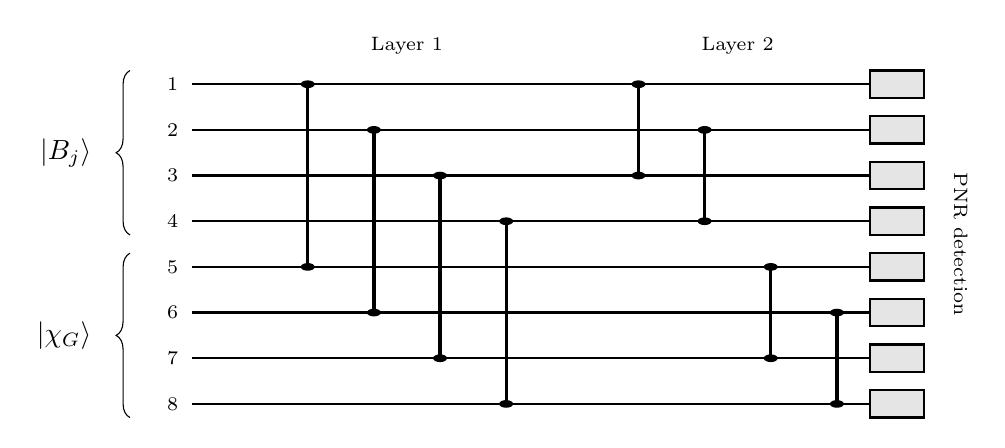
\begin{tikzpicture}[xscale=1.05,yscale=0.58,>=Latex]
  \foreach \y in {1,...,8} {
    \draw[thick] (0,9-\y) -- (8.2,9-\y);
    \node[left] at (-0.05,9-\y) {\scriptsize \(\y\)};
    \draw[thick,fill=black!10] (8.2,9-\y-0.3) rectangle (8.85,9-\y+0.3);
  }
  \node[rotate=-90] at (9.3,4.5) {\scriptsize PNR detection};
  \draw[decorate,decoration={brace,amplitude=5pt}] (-0.75,4.7) -- (-0.75,8.3);
  \node[left] at (-1.1,6.5) {\(\ket{B_j}\)};
  \draw[decorate,decoration={brace,amplitude=5pt}] (-0.75,0.7) -- (-0.75,4.3);
  \node[left] at (-1.1,2.5) {\(\ket{\chi_G}\)};
  \foreach \a/\b/\x in {1/5/1.4, 2/6/2.2, 3/7/3.0, 4/8/3.8} {
    \draw[very thick] (\x,9-\a) -- (\x,9-\b);
    \fill (\x,9-\a) circle (2.4pt);
    \fill (\x,9-\b) circle (2.4pt);
  }
  \foreach \a/\b/\x in {1/3/5.4, 2/4/6.2, 5/7/7.0, 6/8/7.8} {
    \draw[very thick] (\x,9-\a) -- (\x,9-\b);
    \fill (\x,9-\a) circle (2.4pt);
    \fill (\x,9-\b) circle (2.4pt);
  }
  \node at (2.6,8.85) {\scriptsize Layer 1};
  \node at (6.6,8.85) {\scriptsize Layer 2};
\end{tikzpicture}
\caption{The attaining eight-mode circuit. Each vertical segment is a
balanced beam splitter applying the matrix \(B\) of \cref{eq:BS} to the two
modes it connects: layer 1 couples \((1,5),(2,6),(3,7),(4,8)\) and layer 2
couples \((1,3),(2,4),(5,7),(6,8)\). Modes \(1\)--\(4\) carry the dual-rail
Bell state, modes \(5\)--\(8\) carry the ancilla \(\ket{\chi_G}\), and every
output mode ends in a photon-number-resolving detector.}
\label{fig:circuit}
\end{figure}

A direct expansion of the four output states gives the conditional success
probabilities
\begin{equation}
  p_{\Phi^+}=p_{\Phi^-}=\frac12,
  \qquad
  p_{\Psi^+}=p_{\Psi^-}=1.
  \label{eq:grice-success}
\end{equation}
Consequently the equal-prior average is
\begin{equation}
  \frac14\left(\frac12+\frac12+1+1\right)=\frac34.
\end{equation}
These conditional probabilities, the induced partition of all \(330\)
four-photon PNR patterns into \(196\) successful and \(134\) inconclusive
outcomes, and the two-layer decomposition of \cref{eq:S} have been verified
symbolically with two independent exact amplitude engines, one based on
matrix permanents and one on creation-operator polynomial expansion; the
verification code and machine-readable certificates accompany this paper as
ancillary files. Thus this finite passive circuit attains the upper bound in
\cref{thm:main}~\cite{Grice2011}.


\section{Discussion}

The proof avoids optimizing a parametrized interferometer. Instead, it assigns
a local success budget to every output mode. Three structures make the budget
possible:

\begin{enumerate}[leftmargin=2em]
\item Exact unambiguity makes successful post-annihilation Fock coordinates
exclusive, so deleting them preserves a genuine residual Gram matrix.
\item Dual-rail structure supplies a product state in the kernel of any single
signal annihilator.
\item Maximal entanglement caps every Bell coefficient of that product state by
one half.
\end{enumerate}

The global theorem then follows from number conservation and one-particle
Parseval identities. Arbitrarily many vacuum modes cannot help because they do
not change the signal trace \(4\) or the ancillary photon number \(2\).
Likewise, an arbitrary two-photon wavefunction cannot evade the proof because it
enters only through the nonnegative local expectations \(q_\ell\) whose sum is
fixed.

Equality in every step imposes strong local conditions. The product-kernel
vector must place all residual diagonal weight on Bell coefficients of squared
magnitude \(1/2\), and the global frame budgets must be saturated. These
conditions may support a classification of all optimal two-photon schemes up
to passive-optical equivalence. The fixed-\(k\) bound also raises the question
of which ancillary photon numbers admit constructions saturating
\cref{eq:kbound}.

\section{Conclusion}

For static passive linear optics, ideal PNR detection, arbitrary finite mode
extensions, and an arbitrary pure ancillary state containing exactly two
photons, the optimal unambiguous dual-rail Bell-state measurement success is
\begin{equation*}
  \boxed{\Pstar=\frac34.}
\end{equation*}
The upper bound is analytic and independent of the number of ancillary or
vacuum modes, while the lower bound is attained by the finite Grice circuit.
The same local argument yields the general fixed-photon-number bound
\(P_{\mathrm{succ}}\le(k+1)/(k+2)\).

\appendix

\section{Parseval identities in one-particle notation}
\label{app:parseval}

Let \(\{\ket{c_\ell}\}_{\ell=1}^m\) be the orthonormal one-particle vectors of
the pulled-back output modes, and let \(P_S,P_A\) be the signal and ancillary
one-particle projectors. Then
\begin{equation}
  t_\ell=\norm{P_Sc_\ell}^2,
  \qquad
  \sum_\ell t_\ell
   =\Tr\!\left(P_S\sum_\ell\ket{c_\ell}\bra{c_\ell}P_S\right)
   =\Tr P_S=4.
\end{equation}
Writing \(r_\ell\) for the annihilator associated with \(P_Ac_\ell\),
\begin{equation}
  \sum_\ell r_\ell^\dagger r_\ell=N_A,
\end{equation}
and therefore
\begin{equation}
  \sum_\ell q_\ell
   =\bra\chi N_A\ket\chi=2.
\end{equation}
These equalities hold for every finite vacuum extension and every passive
unitary.

\section{Equality conditions in the per-mode argument}
\label{app:equality}

Equality in \cref{eq:permode} requires equality in
\begin{equation}
  \frac{t_\ell}{2}
   \le\sum_jf_{j\ell}w_j
   \le\frac12\sum_jf_{j\ell}.
\end{equation}
Hence every index with \(f_{j\ell}>0\) must satisfy \(w_j=1/2\), and the chosen
product-kernel vector must satisfy \(z^\dagger F_\ell z=0\). The Grice witness
saturates the resulting per-mode budget in every output mode. A full
classification would additionally need compatibility of these equality
conditions across all \(\ell\) with a common ancilla and common unitary.

\section*{Data and code availability}

The exact symbolic verification code, the complete PNR-pattern partition for
the attaining circuit, machine-readable certificates, and replay
instructions are distributed as ancillary files with this paper.

\section*{Acknowledgments}

OpenAI's GPT-5.6 Sol Pro was used as an AI research assistant. The model
contributed to the development of the conditional-Gram upper-bound
argument, the fixed-photon-number extension, exact checks of the
attaining construction, literature exploration, manuscript preparation,
and Lean formalization. Model outputs were treated as provisional and
were retained only when supported by the explicit derivations or exact
certificates associated with this work. The author assumes full
responsibility for all claims and conclusions.

\begin{thebibliography}{99}

\bibitem{Bartolucci2023}
S.~Bartolucci \emph{et al.},
``Fusion-based quantum computation,''
\emph{Nature Communications} \textbf{14}, 912 (2023),
\href{https://doi.org/10.1038/s41467-023-36493-1}{doi:10.1038/s41467-023-36493-1}.

\bibitem{Vaidman1999}
L.~Vaidman and N.~Yoran,
``Methods for reliable teleportation,''
\emph{Physical Review A} \textbf{59}, 116--125 (1999),
\href{https://doi.org/10.1103/PhysRevA.59.116}{doi:10.1103/PhysRevA.59.116}.

\bibitem{Lutkenhaus1999}
N.~L\"utkenhaus, J.~Calsamiglia, and K.-A.~Suominen,
``Bell measurements for teleportation,''
\emph{Physical Review A} \textbf{59}, 3295--3300 (1999),
\href{https://doi.org/10.1103/PhysRevA.59.3295}{doi:10.1103/PhysRevA.59.3295}.

\bibitem{Calsamiglia2001}
J.~Calsamiglia and N.~L\"utkenhaus,
``Maximum efficiency of a linear-optical Bell-state analyzer,''
\emph{Applied Physics B} \textbf{72}, 67--71 (2001),
\href{https://doi.org/10.1007/s003400000484}{doi:10.1007/s003400000484}.

\bibitem{Grice2011}
W.~P. Grice,
``Arbitrarily complete Bell-state measurement using only linear optical elements,''
\emph{Physical Review A} \textbf{84}, 042331 (2011),
\href{https://doi.org/10.1103/PhysRevA.84.042331}{doi:10.1103/PhysRevA.84.042331}.

\bibitem{Ewert2014}
F.~Ewert and P.~van Loock,
``3/4-efficient Bell measurement with passive linear optics and unentangled ancillae,''
\emph{Physical Review Letters} \textbf{113}, 140403 (2014),
\href{https://doi.org/10.1103/PhysRevLett.113.140403}{doi:10.1103/PhysRevLett.113.140403}.

\bibitem{Bayerbach2023}
M.~J. Bayerbach, S.~E. D'Aurelio, P.~van Loock, and S.~Barz,
``Bell-state measurement exceeding 50\% success probability with linear optics,''
\emph{Science Advances} \textbf{9}, eadf4080 (2023),
\href{https://doi.org/10.1126/sciadv.adf4080}{doi:10.1126/sciadv.adf4080}.

\bibitem{Hauser2024}
N.~Hauser, M.~J. Bayerbach, S.~E. D'Aurelio, R.~Weber, M.~Santandrea,
S.~P. Kumar, I.~Dhand, and S.~Barz,
``Boosted Bell-state measurements for photonic quantum computation,''
\emph{npj Quantum Information} \textbf{11} (2025),
\href{https://doi.org/10.1038/s41534-025-00986-2}{doi:10.1038/s41534-025-00986-2}.

\bibitem{Zaidi2013}
H.~A. Zaidi and P.~van Loock,
``Beating the one-half limit of ancilla-free linear optics Bell measurements,''
\emph{Physical Review Letters} \textbf{110}, 260501 (2013),
\href{https://doi.org/10.1103/PhysRevLett.110.260501}{doi:10.1103/PhysRevLett.110.260501}.

\bibitem{Olivo2018}
A.~Olivo and F.~Grosshans,
``Ancilla-assisted linear optical Bell measurements and their optimality,''
\emph{Physical Review A} \textbf{98}, 042323 (2018),
\href{https://doi.org/10.1103/PhysRevA.98.042323}{doi:10.1103/PhysRevA.98.042323}.

\bibitem{Bianchi2025}
L.~Bianchi, C.~Marconi, and D.~Bacco,
``Bell state measurements in quantum optics: a review of recent progress and open challenges,''
\href{https://arxiv.org/abs/2509.18756}{arXiv:2509.18756} (2025; updated 2026).

\bibitem{Laha2026}
P.~Laha and P.~van Loock,
``Auxiliary Schmidt Rank as a Resource for Photonic Bell Measurements,''
\href{https://arxiv.org/abs/2606.24591}{arXiv:2606.24591} (2026).

\end{thebibliography}

\end{document}
